\documentclass[openright, a4paper]{article}
\usepackage{graphicx}
\usepackage{kotex}
\usepackage{minted}
\usepackage{setspace}
\usepackage{underscore}
\usepackage{caption}
\usepackage[margin=3cm]{geometry}
\newcommand{\code}[1]{\texttt{#1}}
\setminted{
    linenos=true,
    autogobble,
}
\newenvironment{longlisting}{\captionsetup{type=listing}}{}
\captionsetup{labelformat=empty,labelsep=none}

\title{2024학년도 컴퓨터구조 Lab Assignment \#5\\
        Cache}

\author{김도영, 선민수}
\date{2024년 5월 30일}

\onehalfspacing
\begin{document}

\maketitle

%%%%%%%%%%%%%%%%%%%%%%%%%%%%%%%%%%%%%%%%%%%%%%%%%%%%%
%                   Introduction                    %
%%%%%%%%%%%%%%%%%%%%%%%%%%%%%%%%%%%%%%%%%%%%%%%%%%%%%

\section{Introduction}
이 과제에서는 Lab Assignment \#4에서 구현했던 파이프라인 CPU에 더해, 주 메모리에 
저장된 값을 임시로 저장하는 캐시를 구현하였다. Lab Assignment \#4까지의 CPU는 
질의를 받으면 한 사이클 내에 해당 메모리의 값을 반환하는, 일종의 '이상화된 
메모리'(Magic memory)를 가정하고 구현되었다. 이번 과제에서는 이러한 이상적 메모리 
모델에서 벗어나, 지연 시간(Latency) 개념을 도입하였다. 즉, 이번 과제에서는 메모리 
접근에 지연 시간이 존재하여 메모리에서 값을 읽어오기까지 CPU의 파이프라인이 
멈춰야 하며, 이는 곧 CPU의 성능 하락으로 이어진다. 이러한 메모리 접근 지연시간을
해결하기 위해 캐시를 도입하고, 다양한 캐시의 구현에 따른 CPU의 성능 변화를 
알아보는 것이 이번 과제의 골자이다.

캐시는 메모리 계층구조(Memory hierachy) 내에서 주 메모리 위, CPU 레지스터 혹은 
상위 계층 캐시 아래에 위치한다. 주 메모리는 용량이 크지만 느리며, CPU 레지스터는 
빠르지만 개수 및 용량이 제한되어 있다. 캐시는 이 둘 사이에 위치하여 최근에 
접근한 값들 또는 이들에 인접한 값들을 미리 저장해두고, CPU의 질의가 있을 
때마다 주 메모리 대신 저장한 값을 전달한다. 캐시는 CPU 레지스터보다는 느리지만 
메모리에 비해서는 월등히 빠르기 때문에, 프로그래머로 하여금 컴퓨터가 용량이 큰 
동시에 빠른, 이상적 주 메모리를 가지고 있는 것 같은 추상화를 제공한다. 

캐시는 그 구현에 따라 직접 사상(Direct-Mapped), 집합 연관 사상(Set-Associative),
완전 연관 사상(Fully-Associative) 캐시로 나눌 수 있다. 직접 사상 캐시는 메모리의
여러 주소가 캐시의 특정 라인에 직접 대응되는 방식의 캐시이다. 이러한 캐시는
구현이 간단하고, 읽기 및 쓰기에 별다른 연산을 요하지 않아 속도가 빠르지만, 
여러 메모리 주소가 캐시의 한 라인에 대응되어 발생하는 충돌(Conflict)의 발생률이
높아 캐시 적중률이 낮아지는 단점이 있다. 집합 연관 사상 캐시는 여러 캐시 라인을
하나의 집합으로 묶어, 특정 메모리 주소에 대한 질의가 들어왔을 때 그 주소에 
해당하는 집합 내 어느 라인에도 데이터를 저장할 수 있도록 만든 캐시이다. 집합
연관 사상 방식은 읽기 및 쓰기 과정에서 집합 내의 각 Way를 탐색해야 하므로
직접 사상 방식에 비해 느리지만, 공간 활용성이 좋아 충돌 발생률이 낮고 캐시 
적중률이 높다는 특징이 있다. 집합 연관 사상 방식에서 더 나아가 집합의 개수를
라인의 개수와 같게 만들어, 쓰기 질의가 들어왔을 때 캐시 내의 아무 라인에나 
데이터를 저장할 수 있게 만든 방식의 캐시를 완전 연관 사상 캐시라 한다. 이번 
과제에서는 직접 사상 및 집합 연관 사상 방식의 캐시를 구현하였다.

%%%%%%%%%%%%%%%%%%%%%%%%%%%%%%%%%%%%%%%%%%%%%%%%%%%%%
%                      Design                       %
%%%%%%%%%%%%%%%%%%%%%%%%%%%%%%%%%%%%%%%%%%%%%%%%%%%%%

\section{Design}
캐시는 단순히 데이터를 저장하고 출력하는 것 뿐만 아니라, CPU의 질의에 응답하여
요청 블록이 현재 캐시에 존재하는지 확인하고, 만약 요청된 블록이 현재 캐시에 
없다면 메모리에 해당 블록이 포함된 라인을 질의하여 메모리가 이에 응답하기까지
기다리는 등, 현재 상태에 따라 다양한 동작을 수행한다. 따라서, 캐시는 내부 상태를
가지고 입력에 따라 상태가 변화하는 유한 상태 기계(Finite State Machine)으로 
구현되며, 이번 과제에서 구현된 캐시는 3개의 상태를 가진 유한 상태 기계로 
구현되었다.

\hfill

{
    \begin{figure}[!h]
        \centering
        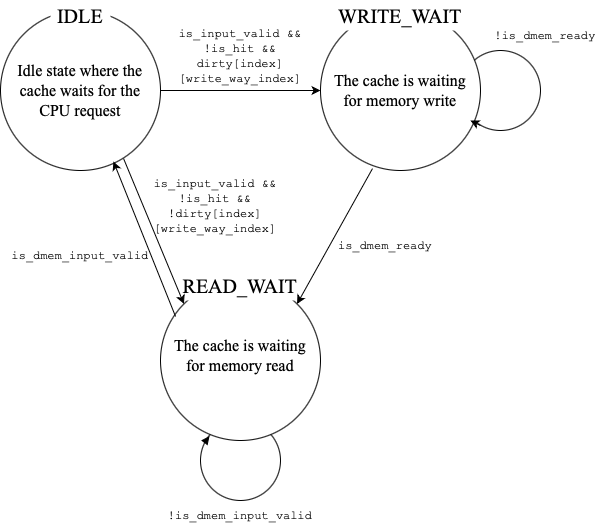
\includegraphics[width=0.75\textwidth]{img/diagram.png}
        \caption{캐시 제어를 위한 유한 상태 기계의 설계}
    \end{figure}
}

\hfill

\begin{description}
  \item[IDLE]상태는 CPU의 요청이 있기 전, 혹은 CPU의 요청을 모두 수행한 후의
  유후 상태를 나타낸다. 캐시는 기본적으로 \code{reset} 신호가 \code{1}일 때,
  이 상태로 초기화된다. IDLE 상태에서, CPU가 요청을 전달하고, 캐시에 요청 대상
  블록이 존재하지 않아 메모리에서 해당 블록을 가져와야 하는 경우 다음 상태로
  전이한다. 만약 요청된 주소에 해당하는 라인이 메모리에서 마지막으로 가져온 이후
  수정되었을(Dirty) 경우 WRITE_WAIT 상태로, 수정되지 않았을 경우 READ_WAIT 상태로
  전이한다.

  \item[WRITE_WAIT]상태는 메모리에 쓰기 요청을 전달하였지만, 메모리가 아직 쓰기가
  완료되었고 다음 요청을 받을 수 있다는 신호(\code{is_ready})를 보내지 않아
  메모리 쓰기 작업이 끝날 때까지 대기하는 상태이다. 만약 해당 신호가 
  \code{1} 이라면 다음 사이클에 READ_WAIT 상태로 전이하며, 아니라면 WRITE_WAIT
  상태에 계속 대기한다.

  \item[READ_WAIT]상태는 메모리에 읽기 요청을 전달하였지만, 메모리가 아직 읽기가
  완료되었고 현재 출력이 유효하다는 신호(\code{is_output_valid})를 보내지 않아
  메모리 읽기 작업이 끝날 때까지 대기하는 상태이다. 만약 해당 신호가 \code{1}
  이라면 다음 사이클에 IDLE 상태로 전이하며, 아니라면 READ_WAIT 상태에 계속 
  대기한다.
\end{description}

캐시는 위와 같은 유한 상태 기계의 상태와 메모리, CPU에서 전달되는 신호에 따라
현재 사이클에서 할 일을 결정한다. 예를 들어, IDLE 상태에서 CPU 쓰기 요청이
전달되었는데, 요청된 블록이 현재 캐시에 존재하는 캐시 적중(Cache Hit) 상황에서는
CPU에서 전달된 데이터를 캐시의 해당 블록에 쓰고 해당 블록이 수정되었음을 
표시한다. 유사하게, READ_WAIT 상태에서 메모리가 현재 출력이 유효하다는 신호가
활성화된 경우, 메모리의 데이터 출력을 캐시의 해당 라인에 쓴다.

본 과제에서 구현한 집합 연관 사상 방식 캐시는 강의 교안의 것을 기반으로
구현하였다. 구현된 캐시의 대략적인 구조도는 다음과 같다.

\hfill

%% TODO: SCHEMATIC IMAGE
{
    \begin{figure}[!h]
        \centering
        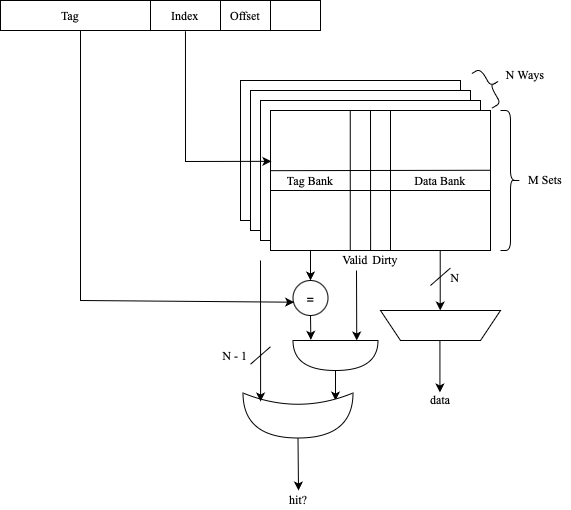
\includegraphics[width=0.75\textwidth]{img/schematic.png}
        \caption{집합 연관 캐시의 구조도}
    \end{figure}
}

\hfill

이전 과제에서 구현한 파이프라인 CPU는 이상적 메모리를 가정하고 구현되었으며,
따라서 메모리가 모든 요청에 1 사이클만에 응답할 것을 가정하였다. 이번 과제에서는
이와 다르게, 메모리 및 캐시가 요청에 바로 응답하지 못할 수도 있다. 때문에, 
CPU에서는 반드시 캐시의 \code{is_ready}, \code{is_hit}, \code{is_output_valid}
신호를 평가하여 파이프라인을 정지할지 결정하여야 한다. 때문에, CPU는 현재
메모리의 상태에 따라 새로운 정지 신호(Stall Signal)을 생성하여 파이프라인의 이전
스테이지에 전달한다. 만약 이러한 신호가 \code{1}인 경우, 캐시가 현재 요청을 모두
처리하고 정지 신호가 다시 \code{0}이 될 때까지 CPU는 대기한다.

\hfill

%%%%%%%%%%%%%%%%%%%%%%%%%%%%%%%%%%%%%%%%%%%%%%%%%%%%%
%                 Implementation                    %
%%%%%%%%%%%%%%%%%%%%%%%%%%%%%%%%%%%%%%%%%%%%%%%%%%%%%

\section{Implementation}

CPU module의 구현은 Lab Assignment \#4까지 구현한 것과 (Design 단락에서 설명한 
부분을 제외하면) 대동소이하며, 따라서 이 보고서에서는 캐시의 구현에 집중하여
설명한다.

\subsection{캐시 상태 전이}

\hfill

\begin{longlisting}
    \begin{minted}[fontsize=\footnotesize]{Verilog}
  always @(*) begin
    case(state)
    `IDLE: begin
      if (is_input_valid && !is_hit)
        next_state = dirty[index][write_way_index] ? `WRITE_WAIT : `READ_WAIT;
      else
        next_state = `IDLE;
    end
    `WRITE_WAIT: next_state = is_dmem_ready ? `READ_WAIT : `WRITE_WAIT;
    `READ_WAIT: next_state = is_dmem_output_valid ? `IDLE : `READ_WAIT;
    default: next_state = `IDLE;
    endcase
  end
    \end{minted}
    \caption{캐시의 다음 상태를 계산하는 조합 논리 회로}
\end{longlisting}

\hfill

캐시의 내부 상태는 위와 같이 IDLE로 초기화되어, CPU의 요청 및 캐시 적중 
여부, 쓰고자 하는 라인의 수정 여부, 메모리의 출력 신호에 따라 WRITE_WAIT,
READ_WAIT 상태로 전이한다.  

\subsection{적중된 Way의 인덱스, 쓰기 인덱스의 계산}

\hfill

\begin{longlisting}
    \begin{minted}[fontsize=\footnotesize]{Verilog}
  // Logic that finds the index of the way that hit
  always @(*) begin
    // Notice that hit_way_index may cause unexpected behaviour when used
    // without testing hit_way_found. Usually you may want to examine is_hit,
    // which essencially is just an alias for hit_way_found, before using
    // hit_way_index.
    hit_way_found = 0;
    hit_way_index = 0;

    for (i = 0; i < NUM_WAYS; i = i + 1) begin
      if (tag == tag_bank[index][i] && valid[index][i]) begin
        hit_way_index = i[WAY_INDEX_LEN - 1: 0]; 
        hit_way_found = 1;
      end   
    end
  end
  
  ...

  // Logic that finds the index of the way to write on
  always @(*) begin
    write_way_found = 0;
    write_way_index = 0;

    for (i = 0; i < NUM_WAYS; i = i + 1) begin
      if (!valid[index][i]) begin
        write_way_index = i[WAY_INDEX_LEN - 1: 0];
        write_way_found = 1;
      end
    end

    if (!write_way_found)
      write_way_index = lru;
  end
    \end{minted}
    \caption{적중된 Way의 인덱스, 쓰기 인덱스를 계산하는 조합 논리 회로}
\end{longlisting}

\hfill

캐시 내에서 \code{hit_way_index}, \code{write_way_index}는 캐시 적중 상황에서
적중한 Way의 인덱스, 캐시 쓰기 요청이 들어오거나 메모리 라인을 캐시에 써야 하는
상황에서 쓰기 대상이 될 Way의 인덱스를 저장하는 레지스터이다. 위 논리 회로는 
기본적으로 캐시의 각 Way를 순회하여, 만약 적중 조건을 만족하는 Way를 찾았을 경우
해당 Way의 인덱스를 \code{hit_way_index}에 저장한다. \code{write_way_index} 또한
비슷하게 캐시의 각 Way를 순회하며 유효하지 않은(\code{!valid}) Way를 먼저 찾는다.
만약 그러한 Way가 없다면, 접근된 지 가장 오랜 시간이 지난(Least Recently Used) 
Way를 찾아 해당 Way의 인덱스를 \code{hit_way_index}에 저장한다.

이때 주의할 점은 \code{hit_way_index}는 만약 적중된 Way를 찾지 못하였을 경우
\code{0}을 저장하며, 이 때문에 캐시 부적중(Cache Miss) 상황에서는 이 \code{0}이
그대로 데이터를 가져오는 인덱스로 사용되어 캐시가 예상치 못한 동작(Unexpected
Behaviour)을 보일 수 있다는 점이다. 따라서, \code{hit_way_index}는 반드시 
\code{hit_way_found}, 혹은 이와 동일한 값을 갖는 별칭인 \code{is_hit}을 테스트한
후에 사용되어야 한다.

\subsection{캐시 쓰기 논리 회로}

\hfill

\begin{longlisting}
    \begin{minted}[fontsize=\footnotesize]{Verilog}

    ...

    end else begin
      state <= next_state;

      if (state == `IDLE && is_input_valid && is_hit && mem_rw) begin
        data_bank[index][hit_way_index][32 * offset +: 32] <= din;
        dirty[index][hit_way_index] <= 1;
      end 
      
      if (state == `READ_WAIT && is_dmem_output_valid) begin
        valid[index][write_way_index] <= 1;
        dirty[index][write_way_index] <= 0;
        tag_bank[index][write_way_index] <= tag;
        data_bank[index][write_way_index] <= dmem_dout;
      end

      ...

    end
    \end{minted}
    \caption{캐시의 태그, 데이터를 업데이트하는 순차 논리 회로}
\end{longlisting}

\hfill

CPU에서 캐시에 쓰기 요청을 보내거나, 메모리에서 읽기 요청에 대한 응답이
도착하였다면 캐시의 태그 저장소(Tag Bank), 데이터 저장소(Data Bank)에 해당 
데이터를 쓰고 유효(Valid), 수정됨(Dirty) 비트를 업데이트해야 한다. 따라서, 캐시는
매 사이클마다 현재 상태와 CPU 요청, 적중 여부, 메모리 신호를 확인하여 필요한 경우
해당 라인의 데이터와 태그를 업데이트한다.

\subsection{LRU 업데이트 및 LRU Way 계산 논리 회로}

\hfill

\begin{longlisting}
    \begin{minted}[fontsize=\footnotesize]{Verilog}
  // Logic that finds the least recently used way in a set 
  always @(*) begin
    lru = 0;
    for (i = 0; i < NUM_WAYS; i = i + 1)
      lru = (lru_bank[index][i] == MAX_LRU) ? i[WAY_INDEX_LEN - 1: 0] : lru;
  end

    ...

      if (state == `IDLE && is_input_valid && is_hit) begin
        for (i = 0; i < NUM_WAYS; i = i + 1) begin
          if (lru_bank[index][i] != MAX_LRU)
            lru_bank[index][i] <= lru_bank[index][i] + 1;
        end
        lru_bank[index][hit_way_index] <= 0;
    \end{minted}
    \caption{LRU Way의 인덱스를 계산하고, LRU 레지스터를 업데이트하는 논리 회로}
\end{longlisting}

\hfill

캐시에서는 요청된 집합의 가장 오래 전에 쓰인 Way(Least Recently Used Way; 이하 
LRU Way로 칭함)를 계산하기 위해, 모든 Way마다 Way가 속한 집합에서의 '순위'를 
저장하는 레지스터, \code{lru_bank}를 가지고 있다. 어떤 Way가 적중할 때마다, 그
Way의 순위는 0으로 재설정되고 해당 집합의 LRU Way를 제외한 나머지 Way들의 순위는 
1씩 늘어난다.

반대로, 요청된 집합의 LRU Way를 찾기 위해, 캐시는 해당 집합의 Way를 모두 순회하여
순위가 \code{MAX_LRU}의 값을 가지는 Way를 찾는다. \code{MAX_LRU}는 
\code{NUM_WAYS - 1}의 값을 가지는 상수로, 어떤 Way의 순위가 \code{MAX_LRU}라는
것은 해당 Way가 LRU Way임을 뜻한다.

쉽게 말해, 영희, 철수, 민수, 길동이 있는 그룹에서 무작위로 한 명씩을 호명한다고
하자. 이때 찾고 싶은 것은 마지막으로 호명된 이후 가장 많은 시간이 지난 사람이다. 
이를 위해 "영희는 1등, 철수는 3등, 민수는 0등, 길동은 2등"과 같은 정보를 
저장해두고, 매 호명마다 호명된 사람은 0등으로, 3등을 제외한 나머지는 등수를 1씩 
올린다. 이후 "호명된 이후 가장 많은 시간이 지난 사람은 누구인가?"와 같은 질의가 
들어오면 현재 3등인 사람을 알려주면 될 것이다. 위 코드는 이와 같은 아이디어를 
구현한다.

%%%%%%%%%%%%%%%%%%%%%%%%%%%%%%%%%%%%%%%%%%%%%%%%%%%%%
%                    Discussion                     %
%%%%%%%%%%%%%%%%%%%%%%%%%%%%%%%%%%%%%%%%%%%%%%%%%%%%%

\section{Discussion}

\subsection{캐시 적중률과 연관성의 관계}

\hfill

직접 사상 캐시는 일반적으로 집합 연관 사상 캐시에 비해 충돌으로 인한 부적중
(Conflict Miss) 횟수가 많고, 따라서 캐시 적중률이 더 낮은 특성을 가진다. 따라서,
캐시 부적중에 의한 파이프라인 정지 시간이 길어져 일반적으로 더 낮은 성능을
갖는다고 알려져 있다. 그렇다면, 실제 구현된 캐시에서 직접 사상 캐시와 집합
연관 사상 캐시의 캐시 적중률은 무엇이 더 높을까? 또한, 집합 연관 사상 캐시에서
Way의 수를 뜻하는 연관성(Associativity)을 계속 늘리면, 캐시 적중률 또한 계속
높아질까?

\hfill

\begin{table*}[!h]
  \centering
  \begin{tabular}{@{}ccccc@{}}
    \hline
    Test Program & Direct-Mapped & 2-Way & 4-Way & 8-Way \\
    \hline
    \code{naive_matmul_unroll} & 0.68 & 0.75 & 0.81 & 0.77 \\
    \code{opt_matmul_unroll} & 0.64 & 0.75 & 0.86 & 0.80 \\
    \hline
  \end{tabular}
  \caption{캐시의 Way 수에 따른 적중률 비교}
  \label{tab:comparison}
\end{table*}

\hfill

실험 결과에 따르면, 4-Way일 때까지는 Way의 개수가 증가할수록 캐시 적중률도 
늘어나는 결과를 보이지만, 4-Way에서 8-Way로 넘어가면서부터 캐시 적중률이 
하락한다. 먼저, 직접 사상 캐시에서 집합 연관 캐시로 넘어가면서 적중률이 상승하는
실험 결과는 Introduction 단락에서 상술한 충돌에 의한 부적중으로 설명할 수 있다. 
즉, 직접 사상 캐시의 가장 큰 문제점인 '다른 메모리 주소라도 같은 캐시 라인에 
대응되면서 원래 있던 블록이 쫓겨나는(Evicted) 현상'이 해결되며 캐시 적중률이 
늘어나는 것으로 해석할 수 있다.

그렇다면, 4-Way 캐시에 비해 8-Way 캐시가 더 낮은 적중률을 보이는 결과는 어떻게
설명할 수 있을까? 이러한 현상은 용량에 의한 부적중(Capacity Miss)으로 설명할 수 
있다. 용량에 의한 부적중이란, 특정 블록이 캐시에 있었으나, 캐시의 용량이 부족하여
새로운 블록을 저장하기 위해 해당 블록이 캐시에서 쫓겨나고, 나중에 다시
원래의 블록을 CPU에서 요청하면 해당 블록이 이미 캐시에서 없어졌기 때문에 발생하는
종류의 부적중을 뜻한다. 물론, 캐시의 연관성이 늘어날수록 충돌에 의한 부적중의 
횟수는 줄어들며, 이는 4-Way까지의 실험 결과로 확인할 수 있다. 하지만, 연관성이 
최적 영역, 즉, 위 실험에서의 4-Way에서 벗어나면 용량에 의한 부적중으로 인해 다시 
적중률이 하락하는 것으로 위 실험 결과를 해석할 수 있다. 

위 실험은 모든 캐시 조합 회로의 지연 시간이 똑같으며, 트랜지스터의 개수 등 다른
제한 사항이 없다는 가정에서 수행했다. 실제 CPU 구현에서는 연관성이 늘어날수록
더 많은 Way를 순회해야 하므로 조합 회로의 복잡도, 혹은 신호 안정화에 걸리는
시간이 늘어날 것이며, 이는 높은 연관성을 가지는 캐시의 성능에 불리하게 작용할 
것이다. 따라서, 캐시 구현에서 연관성은 높을수록 무조건 좋은 것이 아닌, 캐시의 
용량, 주로 수행되는 프로그램의 메모리 접근 패턴, 캐시의 한 라인당 블록의 개수 등
여러 인자를 고려하여 결정되어야 하는 값임을 알 수 있다.

\hfill

\subsection{교체 정책}

\hfill

교체 정책(Replacement Policy)란, 집합 연관 사상 캐시에서 이미 집합 내 모든 Way가
메모리 라인에 의해 점유되고 있으며, 새로운 캐시 라인이 들어와 이미 있는 라인들
중 하나를 쫓아내야 할 때 어떤 것을 쫓아내 새로운 것으로 교체할 지에 대한 
정책이다. 교체 정책에는 가장 최근에 사용된 것을 제외하고 아무 Way나 선택하는 
정책, 가장 먼저 들어간 Way를 교체하는 정책, 사용 횟수가 가장 적은 Way를 교체하는
정책 등이 있으나, 이번 과제에서는 구현이 간단한 편이며 좋은 성능을 보여주는
LRU 교체 정책을 이용해 구현하였다.

LRU 교체 정책은, 한 집합에 존재하는 Way들 중 마지막으로 사용된 지 가장 오랜 
시간이 지난 Way를 새로운 라인으로 교체하는 정책이다. LRU 교체 정책을 구현하기
위해서는, 각 Way마다 가장 마지막으로 언제 쓰였는지를 추적하는 레지스터가 
필요하다. 또한, 캐시 쓰기가 일어날 때마다 집합을 순회하여 가장 사용된 지 오래된
Way를 찾는 과정이 필요하다. LRU 교체 정책에 대한 더 자세한 구현 설명은 
Implementation 단락, 'LRU 업데이트 및 LRU Way 계산 논리 회로'에서 하였다. 

\hfill

\subsection{캐시를 활용한 행렬곱 연산의 최적화}

\hfill

컴퓨터에서 2차원 이상의 행렬은 일반적으로 선형적 자료구조로 바뀌어, 각 행이
메모리 상의 연속된 주소를 가지게 된다. 따라서, 일반적인 $n \times n$ 
정사각행렬의 행렬곱 식

\begin{equation}
  C_{ij} = \sum\limits_{k=1}^nA_{ik}B_{kj}
\end{equation}

을 그대로 구현하면 행렬 $B$의 원소들은 메모리 주소를 뛰어넘으며 참조되게 되고,
이는 캐시 적중률에 중요한 메모리 참조의 지역성을 낮춘다. 그렇다면, 행렬곱 
연산에서 메모리 참조의 지역성을 늘려, 즉, 이미 참조한 바 있는 원소들 주변의
원소들을 먼저 참조하여, 행렬곱 연산을 더 효율적으로 수행할 수 있는 방법에는
무엇이 있을까?

한 가지 방법으로는 정사각행렬을 여러개의 타일(Tile)으로 나누어, 각각의 타일에 
대해 행렬곱 연산을 수행한 결과값을 다시 연산해 최종 결과값을 계산하는 방법이
있다. 해당 알고리즘(Tiled Matrix Multiplication, or \code{opt_matmul_unroll})을
구현한 프로그램과 쉽게 생각할 수 있는 알고리즘(Naive Matrix Multiplication, or 
\code {naive_matmul_unroll})을 여러 캐시 구현에서 실행한 결과 얻은
총 CPU 사이클 수는 다음과 같다.

\hfill

\begin{table*}[!h]
  \centering
  \begin{tabular}{@{}ccccc@{}}
    \hline
    Test Program & Direct-Mapped & 2-Way & 4-Way & 8-Way \\
    \hline
    \code{naive_matmul_unroll} & 70520 & 50742 & 34383 & 38746 \\
    \code{opt_matmul_unroll} & 75835 & 53489 & 29947 & 36128 \\
    \hline
  \end{tabular}
  \caption{캐시의 Way 수 및 알고리즘에 따른 실행 사이클 수 비교}
  \label{tab:comparison}
\end{table*}

\hfill

실험 결과, 캐시의 연관성이 충분히 높지 않은 경우(직접 사상, 2-Way 집합 연관 
사상) \code{naive_matmul_unroll}이 더 좋은 성능을 보여주나, 캐시의 연관성이
높아지면 \code{opt_matmul_unroll}이 더 좋은 성능을 보이는 것을 확인할 수 있다.
이는 캐시 연관성이 충분히 높지 않으면, 충돌으로 인한 부적중에 의해 프로그램의 
높은 지역성이 더 좋은 성능으로 이어지지 않음을 의미한다.

\hfill

%%%%%%%%%%%%%%%%%%%%%%%%%%%%%%%%%%%%%%%%%%%%%%%%%%%%%
%                    Conclusion                     %
%%%%%%%%%%%%%%%%%%%%%%%%%%%%%%%%%%%%%%%%%%%%%%%%%%%%%

\section{Conclusion}

\hfill

이번 과제에서는 이전 과제에서 구현하였던 파이프라인 CPU에, 메모리 참조의 지연
시간을 낮출 수 있는 캐시 메모리를 추가로 구현하고, 각각의 캐시 구현이 가지는 
장단점과 캐시 활용에 최적화된 알고리즘, 캐시의 교체 정책 등과 같은 주제에 대해
탐구해 보았다. 이번 과제를 통해, 캐시는 용량이 크지만 지연 시간이 긴 주 메모리와
용량이 작지만 지연 시간이 짧은 CPU 레지스터 사이에서 일종의 완충 작용을 해
빠르고 큰 메모리 모델을 프로그래머에게 제공함을 알 수 있었다. 또한, 직접 사상,
집합 연관 사상, 완전 연관 사상과 같은 다양한 캐시 구현에 대해 비교해보고, 각각의
캐시 구현에는 일종의 Tradeoff가 있으며 이러한 Tradeoff 사이에서 최적의 구현을
찾는 것이 중요함을 알 수 있었다. 또한, LRU 캐시 교체 정책을 실제로 구현해보며,
집합 연관 사상 캐시에 필수적인 캐시 교체 정책이 어떻게 구현되는지 알 수 있었다.
마지막으로, 두 가지 방식으로 구현된 행렬곱 알고리즘을 각각의 캐시 구현들에서
실행시켜보며 캐시 적중률을 늘리는 데 필수적인 메모리 참조의 지역성을 최대화한
알고리즘이란 무엇인지를 탐구하였다.

이번 과제에서는 그간 가정했었던 이상화된 메모리 구현에서 벗어나 메모리 참조
및 역참조에 지연 시간이 존재하는, 보다 실제와 가까운 메모리 구현을 이용하였다.
하지만, 여러 캐시를 구현하며 보다 실제와 가까운 시뮬레이션에 필수적인 조합 논리
회로의 안정화에 걸리는 지연 시간이 시뮬레이션에 포함되지 않아, 연관성이 높은
캐시에 편향된 결과를 얻었다. 연관성이 높은 캐시의 경우 (일반적으로) IPC가 더
높을 수는 있지만, 명령어의 실행에 더 적은 사이클이 걸림이 실제로 실행 시간이
더 빠름을 의미하지는 않기 때문에, 이런 부분을 시뮬레이션에 포함한다면 더 정확한
시뮬레이션이 가능할 것이다.

\hfill

\end{document}